\chapter{Pacotes de Laboratório}
\label{cp:pacotes}
No âmbito da Engenharia de Software Experimental, diversas pesquisas, técnicas e ferramentas têm sido  desenvolvidos para avaliar modelos ou otimizar soluções. Porém, tais recursos ou informações isoladas não formam um corpo de conhecimento consistente, então tornando necessário compartilhá-los entre os grupos de pesquisa por meio do uso de pacotes de laboratório.

A condução de experimentos controlados e suas respectivas replicações são organizadas em um \textit{framework} proposto por~\citeauthoronline{mendoncca2008framework}~(\citeyear{mendoncca2008framework}). O nível de experiência do condutor do experimento, tanto no papel de experimentador quanto de replicador, influencia a qualidade do estudo experimental e deve ser considerada na análise do experimento (talvez como uma ameaça). O conjunto de informações obtido a partir da execução do processo experimental compõe uma nova instância de pacote de laboratório~\cite{Garcia08}.

Diversos pesquisadores relatam dificuldades na revisão de pacotes de laboratório, como problemas no compartilhamento de conhecimento entre grupos de pesquisa devido à falta de padronização para a integração de um conhecimento novo e/ou isolado ao conhecimento comum~\cite{Scatalon11}. Desse modo, é imprescindível a definição e a construção de um pacote de laboratório com o uso de uma estrutura de simples compreensão. O uso de ontologias para sua estruturação é uma alternativa para facilitar a transferência de conhecimento inter e intra-grupos. A \textit{ExperOntology} foi proposta para a organização de Pacotes de Laboratório e é descrita na Seção~\ref{exper}.

\section{Modelo para Melhoria da Experimentação}
\label{fire}

\citeauthoronline{mendoncca2008framework}~(\citeyear{mendoncca2008framework}) apresentaram um modelo para o processo de experimentação (FIRE – \textit{Framework for Improving the Replication of Experiments}), apresentado na Figura~\ref{image:fire}, que objetiva o gerenciamento do conhecimento e a melhoria de replicações de experimentos controlados em Engenharia de Software.

\begin{figure}[!htb]
\centering
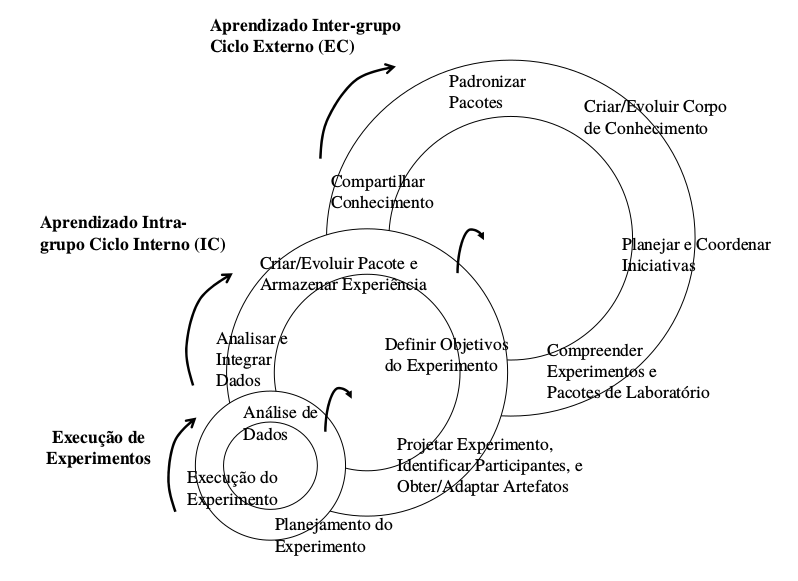
\includegraphics[width=\textwidth]{images/fire.png}
\caption{Ciclos do processo \textit{FIRE}~\cite{mendoncca2008framework}.}\label{image:fire}
\end{figure}

Inicialmente, o ciclo de \textit{Execução do Experimento} corresponde à execução do experimento em estudo. O ciclo de \textit{Aprendizado Intra-Grupo} representa o aprendizado, empacotamento e planejamento de novos experimentos por um mesmo grupo de pesquisadores, visando a construir um corpo de conhecimento local. As atividades desse ciclo consistem em:

\begin{itemize}
\item Definição das metas do experimento.
\item Planejar o experimento, identificar participantes e obter artefatos para a preparação do experimento.
\item Execução do experimento.
\item Instanciação e evolução de Pacotes de Laboratório, armazenando a experiência adquirida.
\end{itemize}

O ciclo de \textit{Aprendizado Inter-Grupo} objetiva a padronização do Pacote de Laboratório, a evolução do pacote de experimentação e o compartilhamento de conhecimento entre os grupos de pesquisa, visa a construir um amplo corpo de conhecimento sobre um tema baseado em replicações executadas por diferentes grupos de pesquisa. As atividades chave
são:

\begin{itemize}
\item Planejamento e coordenação das atividades experimentais entre grupos.
\item Compreensão dos pacotes de laboratório e dos resultados experimentais inter-grupo.
\item Compartilhamento e consolidação do aprendizado com outros grupos.
\item Padronização do conhecimento adquirido pelos grupos de pesquisa.
\item Criação e aprimoramento do corpo de conhecimento.

\end{itemize}

A externalização e internalização do conhecimento na forma de pacotes de laboratório e a concretização do conhecimento externo aos pacotes de laboratório são os pontos críticos do processo \textit{FIRE}. A ausência de diretrizes que apoiem o registro e manutenção de informações explícitas, e a referencia de pacotes de laboratório como corpo de informação explícita sobre um experimento para alcançar uniformidade necessária entre replicações são mencionados na literatura. Entretanto, o \textit{FIRE} não aborda como solucionar tais problemas, assim como não indica outros mecanismos que possam apoiar de modo adequado a evolução do conhecimento~\cite{Garcia06}.


%%%%%%%%%%%%
\section{\textit{ExperOntology}}
\label{exper}
Na Ciência da Computação, o termo ontologia foi introduzido inicialmente por~\citeauthoronline{gruber1995toward}~(\citeyear{gruber1995toward}), que a definiu como ``uma especificação explícita de uma conceitualização''. Posteriormente, uma reformulação foi proposta por~\citeauthoronline{borst1997construction}~(\citeyear{borst1997construction}) acrescentando a perspectiva colaborativa: ``Uma ontologia é uma especificação formal e explícita de uma conceitualização compartilhada''. Quando representado de maneira formal, o corpo do conhecimento se baseia em uma conceitualização explícita ou implícita, sendo composto por objetos, conceitos, outras entidades e as suas relações existentes na área de interesse. Tal conceitualização é considerada uma visão simplificada e abstrata do mundo representado para atingir algum dado objetivo~\cite{rautenberg2016processo}. 
Adicionalmente, uma ontologia é uma especificação formal explícita de uma conceitualização compartilhada, definindo parte de um domínio por meio de termos relevantes e seus respectivos relacionamentos, cuja estruturação é baseada por determinadas regras. 


\citeauthoronline{Garcia08}~(\citeyear{Garcia08}) propõem o uso de uma ontologia para apoiar a atividade de \textit{Empacotamento} no contexto de Engenharia de Software, a qual descreve os conceitos que compõem um pacote de laboratório para experimentos controlados, chamada \textit{ExperOntology}, apresentada em seu nível de abstração mais alto na Figura~\ref{fig:onto01}.


A \textit{ExperOntology} baseia-se no conhecimento de pesquisadores e na experiência em condução de experimentos controlados, principalmente na avaliação das técnicas V\&V (Validação e Verificação). É composta por dois níveis de refinamento, sendo que o primeiro se refere aos principais conceitos de experimento controlado, enquanto o segundo trata do refinamento dos conceitos e do pacote de laboratório. Na condução de um experimento original, é gerado um pacote de laboratório, assim como no processo de replicação.

\begin{figure}[!ht]
\centering
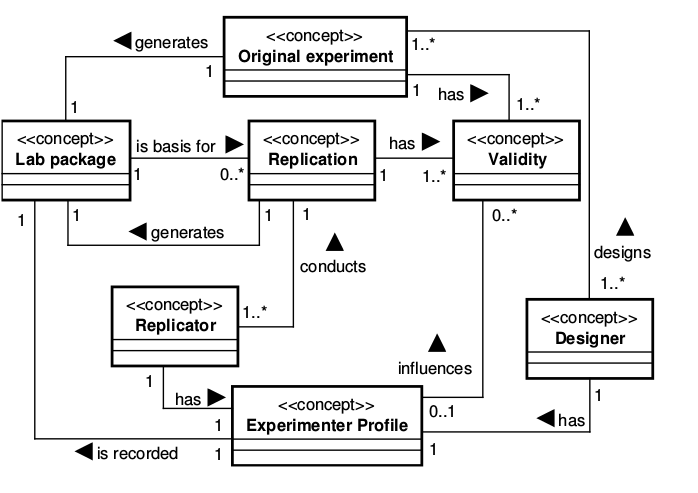
\includegraphics[width=0.9\textwidth]{images/controlados.png}
\caption{Ontologia para Experimentos Controlados~\cite{Garcia08}.}\label{fig:onto01}
\end{figure}

A ontologia proposta por~\citeauthoronline{Garcia08}~(\citeyear{Garcia08}) visa a definir o principais conceitos de experimentos controlados desde a fase de definição até a análise de resultados, sendo importante ressaltar a evolução do experimento e o uso de pacotes de laboratório para armazenamento. 

\begin{figure}[!htb]
\centering
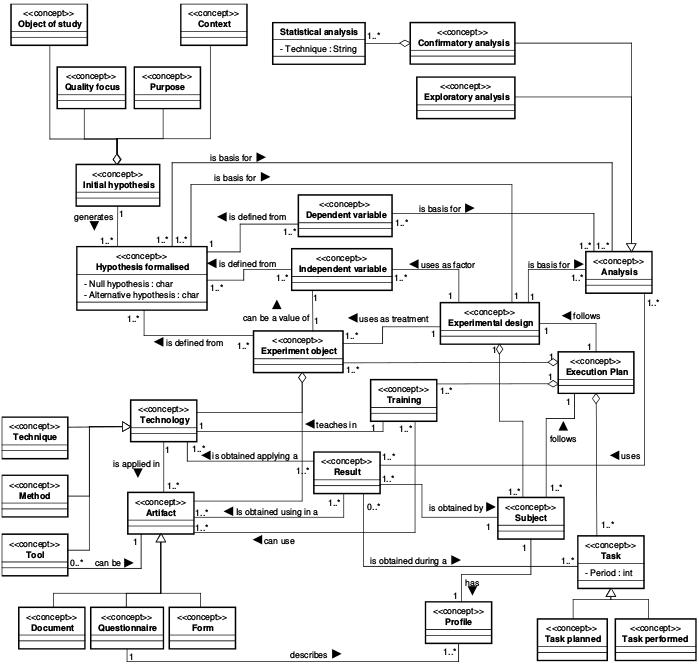
\includegraphics[width=\textwidth]{images/onto.png}
\caption{Ontologia para Pacotes de Laboratório~\cite{Garcia08}.}\label{fig:onto02}
\end{figure}

Na Figura~\ref{fig:onto02} são definidos os conceitos para um pacote de laboratório. Inicialmente, a hipótese inicial de um experimento controlado é definida, sendo constituída pelo objeto de estudo, de acordo com o propósito, sob o foco da qualidade e um contexto específico. Um exemplo de utilização de como um conceito instanciado é utilizado em múltiplas  fases do processo de um experimento, é o conceito \textit{Hipótese Formalizada}:

\begin{itemize}
\item Na atividade \textit{Definição}, a medida que o objetivo do experimento é definido, a base para formulação das hipóteses também é estabelecida, incluindo a \textit{Hipótese Inicial}.
\item Durante a atividade Planejamento, servirá de base para a criação das \textit{Hipóteses Formalizadas} (Hipótese Nula e Hipótese Alternativa). Após a criação das \textit{Hipóteses Formalizadas}, o experimentador estabelece a \textit{Variável Independente} e \textit{Variável Dependente}.
\item Durante a atividade \textit{Operação}, os tratamentos são aplicados aos sujeitos, ou seja, o experimento tem sua execução iniciada.
\item Após o término da execução, ainda na atividade \textit{Operação}, é conveniente que o experimentador aplique uma validação dos dados. Isso ocorre por meio da verificação e validação dos dados informados pelos participantes, para que os resultados do experimento sejam válidos, e para tanto, as \textit{Hipóteses Formalizadas} são ser consultadas.
\end{itemize}


Em seguida, na atividade \textit{Análise e Interpretação}, durante os \textit{Testes de Hipóteses}, as \textit{Hipóteses Formalizadas} passam por avaliação para que seja verificado qualquer possibilidade de rejeição de uma hipótese nula. Hipóteses e conclusões são armazenadas no pacote de laboratório~\cite{Pucci2014}. 

Todos os conceitos apresentados devem ser mantidos no Pacote de Laboratório. Quando se uma ferramenta computacional como apoio ao \textit{Empacotamento}, os conceitos podem ser persistidos em uma base de dados ou outro meio equivalente.


\section{Bancos de Dados Não-Relacionais}

Diversas tecnologias para armazenamento de dados têm sido propostas para a persistência de dados, como os Sistemas Gerenciadores de Banco de Dados (\textit{SGBDs}).

O modelo relacional de dados tem sido utilizado em larga escala desde a sua criação. Esse modelo tem como característica a utilização de tabelas e tuplas para o armazenamento de dados, assim como o uso de chaves primárias para garantia a unicidade (identificação única de elementos de dados)~\cite{brito2010bancos}.

Mediante o crescente número de aplicações, o volume de dados tem aumentado exponencialmente nos últimos anos, e com tal crescimento limitações do modelo relacional têm ficado evidente, principalmente quanto à eficiência na recuperação de dados e escalabilidade~\cite{toth2011abordagem}. Para este projeto, a principal limitação é a restrição de estruturas de tabelas pré-definidas, com seus respectivos atributos, trata-se de um fator limitante, pois experimentos controlados podem ter variações nos dados tratados, difícil de ser acomodados em uma estrutura relacional.

Como alternativa, há soluções tecnológicas que priorizam flexibilidade quanto ao armazenamento, desse modo, não empregam regras presentes no modelo relacional tradicional. Um dessas alternativas é o Modelo Não-Relacional (NoRel), cujo objetivo não é substituir o modelo relacional, mas utilizá-lo em casos em que seja mais vantajoso admitindo a falta de rigidez nas estruturas de dados, como em ambientes de Big Data. Alguns representantes de base não-relacionais são: Cassandra~\cite{cassandra2014apache}, Dynamo~\cite{sivasubramanian2012amazon}, MongoDB~\cite{banker2011mongodb} e BigTable~\cite{chang2008bigtable}.

Devido à inexistência de regras para a organização dos seus dados, diversas categorias de sistemas de banco de dados não-relacionais tem sido desenvolvidas, os principais são detalhados a seguir.

\begin{itemize}
\item Orientados a Colunas (\textit{Column}): é a categoria que mais se aproxima do modelo relacional, porém todas as suas operações são voltadas para as colunas, ao invés das tuplas, como no modelo relacional. O seu grande diferencial está na facilidade de inserção de novas colunas, ou seja, novos atributos com o sistema já em operação, conforme se tornarem necessários, sem apresentar problemas de esquema ou redundância de dados~\cite{vaish2013getting}.

\item Armazenamento em Documentos (\textit{Document}): nessa categoria cada item é armazenado em um novo arquivo, em geral sua organização é feita por meio de estruturas chamadas \textit{Coleções} as quais são equivalentes as tabelas no modelo relacional, não possuem qualquer esquema, dois objetos de uma mesma coleção podem ter atributos diferentes, o que permite grande flexibilidade, sendo que cada registro é um arquivo. Os principais formatos de arquivos são JSON, XML, BSON e YAML~\cite{vaish2013getting}.

\item Armazenamento Chave/Valor (\textit{Key/Value}): também muito semelhante à categoria anterior (\textit{Document}), porém seu armazenamento é feito com uso de uma chave, assemelhando-se a uma tabela \textit{Hash}, ou um \textit{array} associativo. Sua grande vantagem é busca por chaves~\cite{vaish2013getting}.

\item Armazenamento em Grafos (\textit{Graph}): esta categoria tem foco nos relacionamentos entre as entidades, que no caso são os nós do grafo, permitindo o uso de múltiplas ligações entre os nós para demonstrar características em comum. Esse modelo pode ser ideal para redes sociais. Uma prática usual é a mescla entre o banco de dados orientado a documentos e o orientado a grafos, tornando não obrigatória a presença de relacionamentos~\cite{vaish2013getting}.

\end{itemize}

\begin{table}[!htb]
\centering
\caption{Banco de Dados Não-Relacional e sua tecnologia de armazenamento.}\label{tab:01}
\begin{tabular}{c|c|c|c|c}
\hline
\textbf{Document} & \textbf{Key-Value} & \textbf{XML} & \textbf{Column} & \textbf{Graph}\\ 
\hline                               
MongoDB & Redis & BaseX & BigTable & Neo4J \\
\hline
CouchDB & Membase & eXist & Haddop/HBase & FlockDB \\
\hline
RavenDB & Voldemort & - & Cassandra & InfiniteGraph \\
\hline
\end{tabular}
\end{table}
\normalsize

Na Tabela~\ref{tab:01} há uma lista sucinta de tecnologias de banco de dados não-relacionais e a respectiva classificação, segundo as classes de armazenamento apresentadas.
Antes de se estabelecer uma comparação entre os modelos, é importante definir conceitos como que deem compor essa comparação, são eles~\cite{toth2011abordagem,brito2010bancos}:

\begin{itemize}
\item Escalonamento: este conceito, no contexto de banco de dados, consiste na capacidade de distribuição tanto horizontal (\textit{scale out}), neste caso a estruturação do sistema é dividida em várias máquinas tanto por parte do banco de dados; quanto vertical (\textit{scale up}), no qual são realizadas melhorias de hardware em relação ao processamento e ao armazenamento.

\item Consistência: refere-se à capacidade de manter os dados de forma íntegra, de modo que evite inconsistências no banco de dados que corrompam os dados armazenados.

\item Disponibilidade: esse quesito se refere à capacidade de acesso do usuário à referida informação, tanto em quesito de velocidade, quanto de solicitação.
\end{itemize}

\begin{table}[!bth]

\centering
\caption{Análise Comparativa do Modelo Relacional e Não-Relacional~\cite{brito2010bancos}.}
\label{tabela:comparativo}
\begin{tabular}{l|p{5.7cm}|p{5.7cm}}
\hline
 & \textbf{Relacional} & \textbf{Não-Relacional} \\ 
\hline                               
\textbf{Escalonamento} & Possível, porém complexo devido à natureza estruturada do modelo, a adição de forma dinâmica e transparente de novos nós no modelo; não é realizada de modo natural. & Uma das principais vantagens desse modelo, por não possuir nenhum tipo de esquema predefinido, o modelo possui maior flexibilidade; o que favorece a inclusão transparente de outros elementos.\\
\hline
\textbf{Consistência} & Ponto mais forte do modelo relacional. As regras de consistência presentes propiciam uma maior grau de rigor quanto à consistência dos dados. & Realizada de modo eventual no modelo: só garante que, se nenhuma atualização for realizada sobre o item de dados, todos os acessos a esse item devolvem o último valor atualizado. \\
\hline
\textbf{Disponibilidade} & Dada a dificuldade de se conseguir trabalhar de forma eficiente com a distribuição dos dados, esse modelo pode não suportar a demanda muito grande de informações do banco. & Outro fator fundamental do sucesso desse modelo. O alto grau de distribuição dos dados propicia que um maior número de solicitações aos dados seja atendida por parte do sistema e que o sistema fique menos tempo não-disponível. \\
\hline
\end{tabular}
\normalsize
\end{table}

Por fim, de modo a esclarecer as reais vantagens e desvantagens do uso de uma base de dados não-relacional, na Tabela~\ref{tabela:comparativo} é apresentado um comparativo com o tradicional modelo relacional analisando os quesitos de consistência, escalonamento e disponibilidade~\cite{brito2010bancos}. 

\section{Considerações Finais}
Como apresentado neste capítulo, a condução de processos experimentais de modo isolado não é capaz de solidificar um corpo de conhecimento, faz-se necessário a avaliação de modelos, técnicas e ferramentas sob diferentes perspectivas e níveis de experiência. Desse modo, foi apresentado o arcabouço de atividades denominado \textit{FIRE}~\cite{mendoncca2008framework}, que visa ao aprimoramento do conhecimento oriundo de experimentos. Adicionalmente, foi apresenta uma ontologia denominada \textit{ExperOntology}, a qual descreve o conjunto de conceitos para a formalização de um pacote de laboratório em experimentos controlados. Porém a qualidade do pacote instanciado está atrelado diretamente à tecnologia utilizada em sua concepção. Desse modo, apresentam-se com grande viabilidade base de dados não-relacionais orientadas a documentos, devido a eliminação de diversos regras de integridade, além de prover maior flexibilidade de dados, em detrimento às bases de dados relacionais.